% -------------------------------------------------------------
% --------------------- LECTURE 11 29/11 ----------------------
% -------------------------------------------------------------
\subsection{Dualizability in the context of topological field theories} % (fold)
\label{sub:back_to_ordinary_tfts}

Given $\Zf:\Bordn\to\Vect$ and $M\in\Bordn$, one can prove that $\Zf(M)$ is a finite dimensional vector space. Specifically, we have that $\dim \Zf (M) = \Zf (M \times S^1)(1)$, where $M \times S^1$ is an $n$ dimensional cobordism from $\emptyset$ to $\emptyset$.
\begin{proof}
    Decompose $M\times S^1$ into two semicircles $M\times [0,1]$. Then it gets mapped by $\Zf$ to $\Vect_k$ in the following manner
% https://q.uiver.app/#q=WzAsMTYsWzAsMCwiXFxlbXB0eXNldCJdLFsyLDAsIk1cXGFtYWxnIE0iXSxbNCwwLCJcXGVtcHR5c2V0Il0sWzEsMSwiXFxwaGFudG9te0R9TVxcdGltZXMgIl0sWzEsMF0sWzEsMl0sWzMsMSwiTVxcdGltZXMiXSxbMywwXSxbMywyXSxbMCwzLCJrXFxjb25nXFxaZihcXGVtcHR5c2V0KSJdLFsyLDMsIlxcWmYoTSlcXG90aW1lc1xcWmYoTSkiXSxbMSwzXSxbNCwzLCJcXFpmKFxcZW1wdHlzZXQpXFxjb25nIGsiXSxbMywzXSxbMiwyXSxbNCwxXSxbMCwxLCJNXFx0aW1lcyBbMCwxXSJdLFswLDksIlxcWmYiLDIseyJjdXJ2ZSI6Mywic3R5bGUiOnsidGFpbCI6eyJuYW1lIjoibWFwcyB0byJ9fX1dLFs5LDEwLCJcXFpmKE1cXHRpbWVzIFswLDFdKSIsMl0sWzMsMTEsIlxcWmYiLDIseyJsYWJlbF9wb3NpdGlvbiI6NjAsIm9mZnNldCI6LTUsInNob3J0ZW4iOnsic291cmNlIjozMCwidGFyZ2V0IjoxMH0sInN0eWxlIjp7InRhaWwiOnsibmFtZSI6Im1hcHMgdG8ifX19XSxbMTAsMTIsIlxcWmYoTVxcdGltZXMgWzAsMV0pIiwyXSxbNiwxMywiXFxaZiIsMix7InNob3J0ZW4iOnsic291cmNlIjozMCwidGFyZ2V0IjoxMH0sInN0eWxlIjp7InRhaWwiOnsibmFtZSI6Im1hcHMgdG8ifX19XSxbMiwxMiwiXFxaZiIsMCx7ImN1cnZlIjotMiwic3R5bGUiOnsidGFpbCI6eyJuYW1lIjoibWFwcyB0byJ9fX1dLFsxLDE0LCIiLDAseyJvZmZzZXQiOjUsImN1cnZlIjo1LCJzdHlsZSI6eyJoZWFkIjp7Im5hbWUiOiJub25lIn19fV0sWzEsMiwiTVxcdGltZXMgWzAsMV0iXSxbNyw4LCIiLDAseyJvZmZzZXQiOi0yLCJjdXJ2ZSI6LTUsInN0eWxlIjp7ImhlYWQiOnsibmFtZSI6Im5vbmUifX19XV0=
\[\begin{tikzcd}[cramped]
    \emptyset & {} & {M\amalg M} & {} & \emptyset \\
    & {\phantom{D}M\times } && M\times & {} \\
    & {} & {} & {} \\
    {k\cong\Zf(\emptyset)} & {} & {\Zf(M)\otimes\Zf(M)} & {} & {\Zf(\emptyset)\cong k}
    \arrow["{M\times [0,1]}", from=1-1, to=1-3]
    \arrow["\Zf"', curve={height=18pt}, maps to, from=1-1, to=4-1]
    \arrow["{\Zf(M\times [0,1])}"', from=4-1, to=4-3]
    \arrow["\Zf"'{pos=0.6}, shift left=5, shorten <=10pt, shorten >=3pt, maps to, from=2-2, to=4-2]
    \arrow["{\Zf(M\times [0,1])}"', from=4-3, to=4-5]
    \arrow["\Zf"', shorten <=10pt, shorten >=3pt, maps to, from=2-4, to=4-4]
    \arrow["\Zf", curve={height=-12pt}, maps to, from=1-5, to=4-5]
    \arrow[shift right=5, curve={height=30pt}, no head, from=1-3, to=3-3]
    \arrow["{M\times [0,1]}", from=1-3, to=1-5]
    \arrow[shift left=2, curve={height=-30pt}, no head, from=1-4, to=3-4]
\end{tikzcd}\]
    %If $V = \Zf(M)$ is finite dimensional, then $\Zf(M \times )
    We claim that the maps will roughly be $k \to V^\vee \otimes V \xrightarrow{evaluate} k$, where the first map sends $1 \mapsto \sum_{i=1}^n f_i\otimes e_i$ where $e_i$ is a basis of $V$ and $f_i$ is the dual basis.
\end{proof}

\begin{defn}
    Let $\Bordnor$ be the category with:
    \begin{itemize}
        \item objects: closed and oriented $(n-1)$-manifolds
        \item morphisms: $\Hom_{\Bordnor} (M,N) = $ orientation preserving diffeomorphism classes of oriented bordisms. i.e. a bordism $(\Sigma, p, \theta_0, \theta_1)$ where $\Sigma$ has an orientation and the diffeomorphism $\de \Sigma \cong \bbar M \amalg N$ is an orientation preserving one.
    \end{itemize}
\end{defn}

\begin{notat}
    We denote with $\bullet_+$ the positively oriented point, i.e. the closed 0-dimensional manifold from where there is an outgoing 1-dimensional bordism. 
    
    We denote with $\bullet_-$ the negatively, i.e. the closed 0-dimensional manifold which is the incoming boundary of a 1-dimensional bordism.
\end{notat}

\begin{ex}[Some objects and morphisms from $\Bord^{\operatorname{or}}_{1,0}$]

\[ 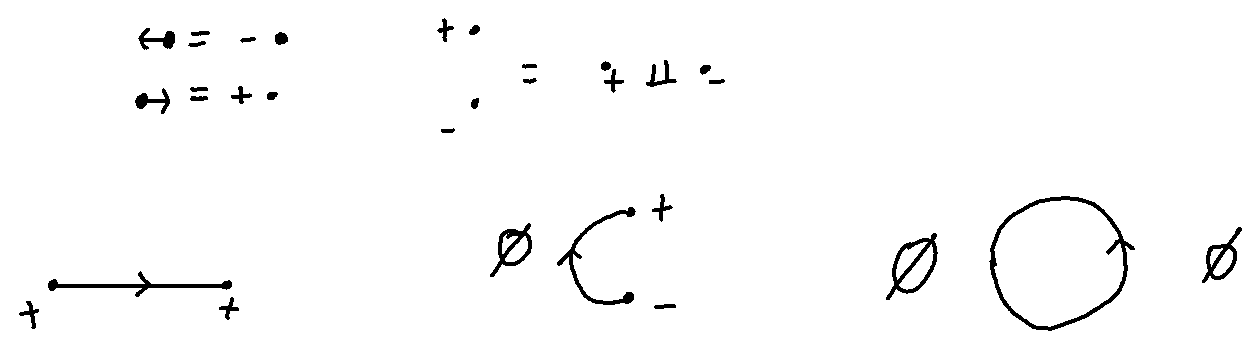
\includegraphics[width=9cm]{images/Lecture 11/1dBORDISM.png}\]
          
\end{ex}
\begin{ex}[Some objects and morphisms from $\Bord^{\operatorname{or}}_{2,1}$]

\[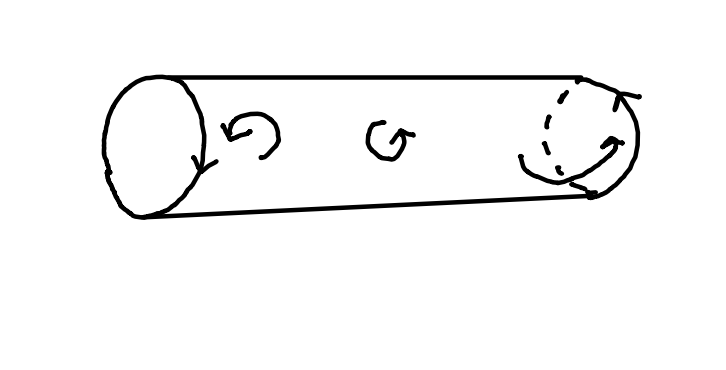
\includegraphics[width=6cm]{images/Lecture 11/2dBORDISM.png} \]
          

    Note that the orientation on the outgoing boundary is opposite to the induced orientation on the incoming one.
\end{ex}

We can also define analogous categories for other tangential structures, e.g. a framing.

\begin{ex}
    In 1 and 2 dimensions...
    %DRAWINGS
\end{ex}

\begin{defn}\label{DefDualObj}
    Let $\cat$ be a monoidal category. A left dual of an object $X \in \cat$ is an object $Y$ together with $ev_X: Y \otimes X \to \unit_\cat$ and $coev_X: \unit_\cat \to X \otimes Y$ such that
    
   % https://q.uiver.app/#q=WzAsMyxbMCwwLCJcXG1hdGhiYnsxfV9cXGNhdFxcb3RpbWVzIFhcXGNvbmcgWCJdLFsxLDEsIlhcXG90aW1lcyBZXFxvdGltZXMgWCJdLFsyLDAsIlhcXG90aW1lc1xcbWF0aGJiezF9X1xcY2F0XFxjb25nIFgiXSxbMCwxLCJjb2V2X1hcXG90aW1lcyBpaWRfWCIsMl0sWzEsMiwiaWRfWFxcb3RpbWVzIGV2X1giLDJdLFswLDIsImlkX1giLDAseyJvZmZzZXQiOi0xLCJzdHlsZSI6eyJoZWFkIjp7Im5hbWUiOiJub25lIn19fV0sWzAsMiwiIiwxLHsib2Zmc2V0IjoxLCJzdHlsZSI6eyJoZWFkIjp7Im5hbWUiOiJub25lIn19fV1d
    \begin{equation}
        \begin{tikzcd} \label{DUAL1}
            {\mathbb{1}_\cat\otimes X\cong X} && {X\otimes\mathbb{1}_\cat\cong X} \\
            & {X\otimes Y\otimes X}
            \arrow["{coev_X\otimes id_X}"', from=1-1, to=2-2]
            \arrow["{id_X\otimes ev_X}"', from=2-2, to=1-3]
            \arrow["{id_X}", from=1-1, to=1-3]
        \end{tikzcd}
    \end{equation}
    and
    
   % https://q.uiver.app/#q=WzAsMyxbMCwwLCJZXFxvdGltZXNcXG1hdGhiYnsxfV9cXGNhdFxcY29uZyBZIl0sWzEsMSwiWVxcb3RpbWVzIFhcXG90aW1lcyBZICJdLFsyLDAsIlxcbWF0aGJiezF9X1xcY2F0XFxvdGltZXMgWVxcY29uZyBZIl0sWzAsMSwiaWRfWVxcb3RpbWVzIGNvZXZfWSIsMl0sWzEsMiwiZXZfWVxcb3RpbWVzIGlkX1kiLDJdLFswLDIsImlkX1kiLDAseyJvZmZzZXQiOi0xLCJzdHlsZSI6eyJoZWFkIjp7Im5hbWUiOiJub25lIn19fV0sWzAsMiwiIiwxLHsib2Zmc2V0IjoxLCJzdHlsZSI6eyJoZWFkIjp7Im5hbWUiOiJub25lIn19fV1d
    \begin{equation}
   \label{DUAL2}
        \begin{tikzcd}
            {Y\otimes\mathbb{1}_\cat\cong Y} && {\mathbb{1}_\cat\otimes Y\cong Y} \\
            & {Y\otimes X\otimes Y }
            \arrow["{id_Y\otimes coev_Y}"', from=1-1, to=2-2]
            \arrow["{ev_Y\otimes id_Y}"', from=2-2, to=1-3]
            \arrow["{id_Y}", from=1-1, to=1-3]
        \end{tikzcd}
    \end{equation}
    The fact that these two diagrams commute is called snake relations. If the diagrams commute, then $X$ is the right dual of $Y$ and $Y$ is the left dual of $X$.
\end{defn}




\begin{rem}
    If $\cat$ is braided, and in particular for us symmetric, any right dual is a left dual and viceversa.
\end{rem}
\begin{notat}
    We denote the dual of an object $X$ with $X^\vee$. Sometimes it is also denoted with $X^\ast$.
\end{notat}
\begin{cor}\label{ImageOfDualStillDual}
    Let $F:\cat\to\dat$ be a monoidal functor. Thanks to monoidal functoriality, the monoidal unit $\unit_\cat$ is sent to $\unit_\dat$ (up to isomorphism), and hence one gets the evaluation map and coevaluation map: $ev_{F(X)}:F(Y)\otimes F(X)\to\unit_\dat\cong F(\unit_\cat)$ and $coev_{F(X)}:F(\unit_\cat)\cong\unit_\dat\to F(X)\otimes F(Y)$. Moreover, the image of a commuting diagram under a functor still commutes (see \ref{FunctorsPreserveCommut}). So, the dual objects are sent to dual objects by monoidal functors and $F(X^\vee)=F(X)^\vee$.
\end{cor}

\begin{ex}
\hfill
\begin{enumerate}
\item Any finite dimensional vector space $V$ has a dual, namely $V^\vee$:
    \begin{align}
        ev_V&: V^\vee \otimes V \to k\\
        coev_V &: k \to V \otimes V^\vee
    \end{align}
    %TODO write what is sent to what.
\item As an exercise try $\Set, \times$
\item $\cat = \Bordnor$.
The point $\bullet_+$ is dualizable with dual $\bullet_-$.
%DRAWING

This construction actually works for any object in $\Bordnor$ (and $\Bordn$).
\end{enumerate}
\end{ex}
\begin{defn}[Dual Morphisms]\label{DualMorph}
    Let $X,Y$ be dualizable objects in a symmetric monoidal category $\cat$ and $f:X\to Y$ be a morphism. The dual morphism is given by $$f^\vee:Y^\vee\xrightarrow{id_{Y^\vee} \otimes coev_X}Y^\vee\otimes X \otimes X^\vee\xrightarrow{id_Y^\vee\otimes f\otimes id_{X^\vee}}Y^\vee\otimes Y\otimes X^\vee\xrightarrow{ev_Y\otimes id_{X^\vee}}X^\vee$$
\end{defn}
\begin{defn}[Picard Groupoid]\label{PicardGroupoid}
    A Picard Groupoid is a symmetric monoidal category where every object is invertible with respect to $\otimes$ (i.e. $\forall A\in\cat, \ \exists A^{-1}$ s.t $ A\otimes A^{-1}\cong\mathbb{1}_\cat$) and every morphism is an isomorphism, and hence it is a groupoid.
\end{defn}

\begin{lem}\label{BordDuals}
    In every bordism category $\Bord_{n,n-1}^{(\orient)}$ every object is dualizable.
\end{lem}
%DRAWING
\begin{lem}\label{DualizableMeansInvertibleNatTrans}
    Given symmetric monoidal categories $\cat$ and $\dat$, symmetric monoidal functors $F,G:\cat\to\dat$ and a symmetric monoidal natural transfromation $\alpha:F\Rightarrow G$, if $X\in\cat$ is dualizable, then $\alpha_X:F(X)\to G(X)$ is invertible.
\end{lem}
\begin{proof}
    We claim that the inverse is given by $\alpha_{(X^\vee)^\vee}$. Following \ref{DualMorph}, $\alpha_{(X^\vee)^\vee}:G(X^\vee)^\vee\to F(X^\vee)^\vee$. Note that $F(X^\vee)=F(X)^\vee$ and thus $F(X^\vee)^\vee=F(X)^{\vee\vee}=F(X)$ and so $\alpha_{(X^\vee)^\vee}:G(X)\to F(X)$. Remember that $ev_X:X^\vee\otimes X\to \unit_\cat$ and $coev_X:\unit_\cat\to X\otimes X^\vee$. We prove that the following diagram commutes
% https://q.uiver.app/#q=WzAsNixbMCwyLCJHKFgpXFxjb25nIEcoWClcXG90aW1lc1xcdW5pdF9cXGRhdCJdLFsxLDUsIkcoWClcXG90aW1lcyBHKFheXFx2ZWUpXFxvdGltZXMgRyhYKSJdLFsxLDAsIkcoWClcXG90aW1lcyBGKFheXFx2ZWUpXFxvdGltZXMgRihYKSJdLFsyLDEsIkcoWClcXG90aW1lcyBHKFheXFx2ZWUpXFxvdGltZXMgRihYKSJdLFsyLDUsIlxcdW5pdF9cXGRhdFxcb3RpbWVzIEcoWClcXGNvbmcgRyhYKSJdLFsyLDQsIlxcdW5pdF9cXGRhdFxcb3RpbWVzIEYoWClcXGNvbmcgRihYKSJdLFswLDEsImlkX3tHKFgpfVxcb3RpbWVzIEcoY29ldl9YKSIsMl0sWzAsMiwiaWRfe0coWCl9XFxvdGltZXMgRihjb2V2X1gpIl0sWzIsMSwiaWRfe0coWCl9XFxvdGltZXNcXGFscGhhX3tYXlxcdmVlfVxcb3RpbWVzXFxhbHBoYV9YIiwxXSxbMiwzLCJpZF97RyhYKX1cXG90aW1lc1xcZXRhX3tYXlxcdmVlfVxcb3RpbWVzIGlkX3tGKFgpfSJdLFsxLDQsIkcoZXZfe1h9KVxcb3RpbWVzIGlkX3tHKFgpfSIsMl0sWzMsNSwiRyhldl9YKVxcb3RpbWVzIGlkX3tGKFgpfSJdLFs1LDQsIlxcZXRhX3tYfSJdLFszLDEsImlkX3tHKFgpfVxcb3RpbWVzIGlkX3tHKFgpfVxcb3RpbWVzIFxcZXRhX1giLDFdXQ==
% https://q.uiver.app/#q=WzAsNixbMiwxLCJHKFgpXFxvdGltZXMgRihYXlxcdmVlKVxcb3RpbWVzIEYoWCkiXSxbMiwyLCJHKFgpXFxvdGltZXMgRyhYXlxcdmVlKVxcb3RpbWVzIEYoWCkiXSxbMSwwLCJHKFgpXFxjb25nIEcoWClcXG90aW1lc1xcdW5pdF9cXGRhdCJdLFsyLDQsIlxcdW5pdF9cXGRhdFxcb3RpbWVzIEYoWClcXGNvbmcgRihYKSJdLFswLDEsIkcoWClcXG90aW1lcyBHKFheXFx2ZWUpXFxvdGltZXMgRyhYKSJdLFswLDQsIlxcdW5pdF9cXGRhdFxcb3RpbWVzIEcoWClcXGNvbmcgRyhYKSJdLFsyLDQsIntpZF97RyhYKX1cXG90aW1lcyBHKGNvZXZfWCl9IiwyXSxbMiwwLCJ7aWRfe0coWCl9XFxvdGltZXMgRihjb2V2X1gpfSJdLFswLDQsIntpZF97RyhYKX1cXG90aW1lc1xcYWxwaGFfe1heXFx2ZWV9XFxvdGltZXNcXGFscGhhX1h9IiwxXSxbMCwxLCJ7aWRfe0coWCl9XFxvdGltZXNcXGFscGhhX3tYXlxcdmVlfVxcb3RpbWVzIGlkX3tGKFgpfX0iXSxbNCw1LCJ7Ryhldl97WH0pXFxvdGltZXMgaWRfe0coWCl9fSIsMl0sWzEsMywie0coZXZfWClcXG90aW1lcyBpZF97RihYKX19IiwxXSxbMyw1LCJ7XFxhbHBoYV97WH19Il0sWzEsNCwie2lkX3tHKFgpfVxcb3RpbWVzIGlkX3tHKFgpfVxcb3RpbWVzIFxcYWxwaGFfWH0iXV0=
\[\begin{tikzcd}
    & {G(X)\cong G(X)\otimes\unit_\dat} \\
    {G(X)\otimes G(X^\vee)\otimes G(X)} && {G(X)\otimes F(X^\vee)\otimes F(X)} \\
    && {G(X)\otimes G(X^\vee)\otimes F(X)} \\
    \\
    {\unit_\dat\otimes G(X)\cong G(X)} && {\unit_\dat\otimes F(X)\cong F(X)}
    \arrow["{{id_{G(X)}\otimes G(coev_X)}}"', from=1-2, to=2-1]
    \arrow["{{id_{G(X)}\otimes F(coev_X)}}", from=1-2, to=2-3]
    \arrow["{{id_{G(X)}\otimes\alpha_{X^\vee}\otimes\alpha_X}}"{description}, from=2-3, to=2-1]
    \arrow["{{id_{G(X)}\otimes\alpha_{X^\vee}\otimes id_{F(X)}}}", from=2-3, to=3-3]
    \arrow["{{G(ev_{X})\otimes id_{G(X)}}}"', from=2-1, to=5-1]
    \arrow["{{G(ev_X)\otimes id_{F(X)}}}"{description}, from=3-3, to=5-3]
    \arrow["{{\alpha_{X}}}", from=5-3, to=5-1]
    \arrow["{{id_{G(X)}\otimes id_{G(X)}\otimes \alpha_X}}", from=3-3, to=2-1]
\end{tikzcd}\]
First of all, the triangle on the top commutes, i.e.
 $(id_{G(X)}\otimes\alpha_{X^\vee}\otimes\alpha_X)\circ(id_{G(X)}\otimes F(coev_X))=id_{G(X)}\otimes G(coev_X)$
 , because of the naturality of $\alpha$. The triangle underneath it also commutes, i.e.
  $id_{G(X)}\otimes\alpha_{X^{\vee}}\otimes\alpha_{X}=(id_{G(X)}\otimes id_{G(X)}\otimes\alpha_{X})\circ (id_{G(X)}\otimes\alpha_{X^{\vee}}\otimes id_{id_{F(X)}})$
    because of the unitality of $id_{G(X)}$ and $id_{F(X)}$.
    Lastly, the bottom trapezoid commutes thanks to the naturality of $\alpha$ and thus the whole big diagram commutes. 
    Consider now first mapping leftwards and successively downwards, i.e. $(G(ev_X)\otimes id_{G(X)})\circ id_{G(X)}\otimes G(coev_X)$, 
    this equals to the identity by one of the two snake relations of dual objects. 
    Take now the other route of the outer diagram, on the right;
     note that $(\alpha_X\vee)\vee=(G(ev_{X})\otimes id_{F(X)})\circ (id_{G(X)}\otimes\alpha_{X^\vee}\otimes id_{F(X)})\circ id_{G(X)}\otimes F(coev_{X})$ 
     by definition (\ref{DualMorph}) and hence the right route on the outer diagram corresponds to
      $\alpha_X\circ(\alpha_{X^\vee})^\vee$. Since the outer diagram commutes we obtain that
       $\alpha_X\circ(\alpha_{X^\vee})^\vee=id_{G(X)}$, i.e. $(\alpha_{X^\vee})^\vee$ is the right inverse of
        $\alpha_X$. One constructs a symmetric diagram by substituting $F$s with $G$s to prove that it is also the left inverse.
\end{proof}
\begin{cor}
    If every object in a symmetric monoidal category $\cat$ is dualizable, then any symmetric monoidal natural transformation between symmetric monoidal functors that have $\cat$ as the source category is invertible since a natural transfomation is invertible if and only if each of its components is invertible. Hence, $\Fun^\otimes(\cat,\dat)$ is a groupoid for any $\dat$ when all objects in $\cat$ are dualizable.
\end{cor}
\begin{cor}\label{TFTsareGRPDS}
    The category of topological field theories $\TFT_{n,n-1}^{or}(\cat)$ is a groupoid.
\end{cor}
\begin{lem}\label{InvDual}
    Any invertible object is dualizable.
\end{lem}
\begin{proof}
    Let $X$ be an invertible object. Then, there must be an $X^{-1}$ such that $X\otimes X^{-1}\cong\mathbb{1}_\cat$, the invertible object is the dual of $X$. The co/evaluation maps become isomorphisms the snake relations hold because if a commutative triangle of isomorphisms commutes in one direction, then it commutes also in the opposite one, i.e. for arbitrary isomorphisms $f,g,h$ such that $f=h\circ g$, it holds that $f^{-1}=(h\circ g)^{-1}=g^{-1}\circ h^{-1}$.
\end{proof}
\begin{lem}\label{InvertibleDualizable}
    A dualizable object is invertible if and only if its co/evaluation maps are isomorphisms.
\end{lem}
\begin{proof}
    $\implies$ directly follows from \ref{InvDual} since any invertible object has as co/evaluation maps isomorphisms. Conversely, suppose that $X$ is a dualizable object and the co/evaluation maps are isomorphisms. Then, there is a $Y\in\cat$ such that $ev_X:Y\otimes X\cong \mathbb{1}$.
\end{proof}
\begin{cor}
    If $\cat$ is a monoidal groupoid, then dualizable objects are invertible.
\end{cor}
\begin{proof}
    Since $\cat$ is a groupoid, then also the co/evaluation maps are isomorphisms. From \ref{InvertibleDualizable} it follows that the dualizable objects are invertible.
\end{proof}
\begin{cor}\label{PicardDualizable}
    A Picard groupoid (\ref{PicardGroupoid}) is equivalently a monoidal groupoid where every object is dualizable.
\end{cor}
\begin{ex}
    The underlying groupoid of $\Bordnor$ is a picard groupoid.
\end{ex}
\begin{notat}
We denote with $\cat^{\cong}$ the underlying groupoid of $\cat$, i.e. the subcategory of $\cat$ where we forget 
about non-invertible morphisms.
\end{notat}
\begin{notat}
We denote with $\cat^{\operatorname{fd}}$ (or sometiimes $\cat^{\operatorname{dualizable}}$) the subcategory of $\cat$ containing only dualizable objects.
We chose 'fd' because it can stand for two things:
\begin{itemize}
    \item 'finite dimensional' since dualizable objects in Vect are finite dimensional vector spaces and in general
    dualizability can be seen as a finiteness condition
    \item 'fully dualizable', a higher-categorical generalization of the notion of dualizability which we encounter
     in the next subsection
\end{itemize}
\end{notat}